\documentclass[12pt]{article}

\usepackage{amsfonts}
\usepackage{graphicx}
\usepackage{amsmath}
\usepackage{mathrsfs}
\usepackage{rotating}
\usepackage{listings}
\usepackage{color}
\usepackage{geometry}
 
\definecolor{codegreen}{rgb}{0,0.6,0}
\definecolor{codegray}{rgb}{0.5,0.5,0.5}
\definecolor{codepurple}{rgb}{0.58,0,0.82}
\definecolor{backcolour}{rgb}{0.95,0.95,0.92}

\lstdefinestyle{mystyle}{
    backgroundcolor=\color{backcolour},   
    commentstyle=\color{codegreen},
    keywordstyle=\color{blue},
    numberstyle=\tiny\color{codegray},
    stringstyle=\color{codepurple},
    basicstyle=\footnotesize,
    breakatwhitespace=false,         
    breaklines=true,                 
    captionpos=b,                    
    keepspaces=true,                 
    numbers=left,                    
    numbersep=5pt,                  
    showspaces=false,                
    showstringspaces=false,
    showtabs=false,                  
    tabsize=2
}
 
\lstset{style=mystyle}

\begin{document}
\begin{center}
\Large{\textbf{ECON 634 Problem Set 7}}\\[3mm]
\large{{Mingyang Li}}\\[1mm]
\today
\end{center}

\begin{enumerate}
\item 
\begin{itemize}
\item The transition function $g$ is $$X_t=g(X_{t-1},X_{t-2},\varepsilon_t,\varepsilon_{t-1},\varepsilon_{t-2};\theta)=\rho_1X_{t-1}+\rho_2X_{t-2}+\phi_1\varepsilon_{t-1}+\phi_2\varepsilon_{t-2}+\varepsilon_t,$$ where $\varepsilon_t\sim\text{N}(0,\sigma_x^2)$.
\item The observation equation $h$ is $$\begin{pmatrix}A_t\\B_t\end{pmatrix}=\begin{pmatrix}h_A(X_t,v_t^A;\theta)\\h_B(X_t,v_t^B;\theta)\end{pmatrix}=\begin{pmatrix}\text{exp}(X_t+\nu_t^A)\\\beta X_t^2+\nu_t^B\end{pmatrix},$$where $\nu_t^A\sim\text{N}(0,\sigma_A^2)$ and $\nu_t^B\sim\text{N}(0,\sigma_B^2)$.
\item The state $S_t$ is $S_t=\lbrace {X_{t-1},X_{t-2},\varepsilon_{t-1},\varepsilon_{t-2}}\rbrace$.
\item The observables $Y_t$ is $Y_t=\begin{pmatrix}A_t\quad B_t\end{pmatrix}'$.
\item The shocks $W_t$ to state variables is $W_t=\begin{pmatrix}\varepsilon_t\end{pmatrix}.$
\item The shocks $V_t$ to observables is $V_t=\begin{pmatrix}\nu_t^A\quad\nu_t^B\end{pmatrix}'.$
\item The parameter vector $\theta$ is $$\theta = \begin{pmatrix}\rho_1 \quad \rho_2 \quad \phi_1 \quad \phi_2 \quad \beta \quad \sigma_x \quad \sigma_A \quad \sigma_B\end{pmatrix}',$$ where $\rho_1$, $\rho_2$, $\phi_1$ and $\phi_2$ are the ARMA(2,2) coefficients, $\beta$ is the coefficient of $X_t^2$ in the observation equation $h_B$, $\sigma_x$ is the standard deviation of the normal distribution to which $\varepsilon_t$ belongs, and $\sigma_A$ and $\sigma_B$ are the standard deviations of the normal distributions to which the measurement errors $\nu_t^A$ and $\nu_t^B$ belong, respectively.
\end{itemize}
\item Please see Appendix B for the code.
\item Please see Appendix A for the code.
The acceptance rate is about 1.7\%. The distributions of parameters are as follows.
\begin{sidewaysfigure}
\centerline{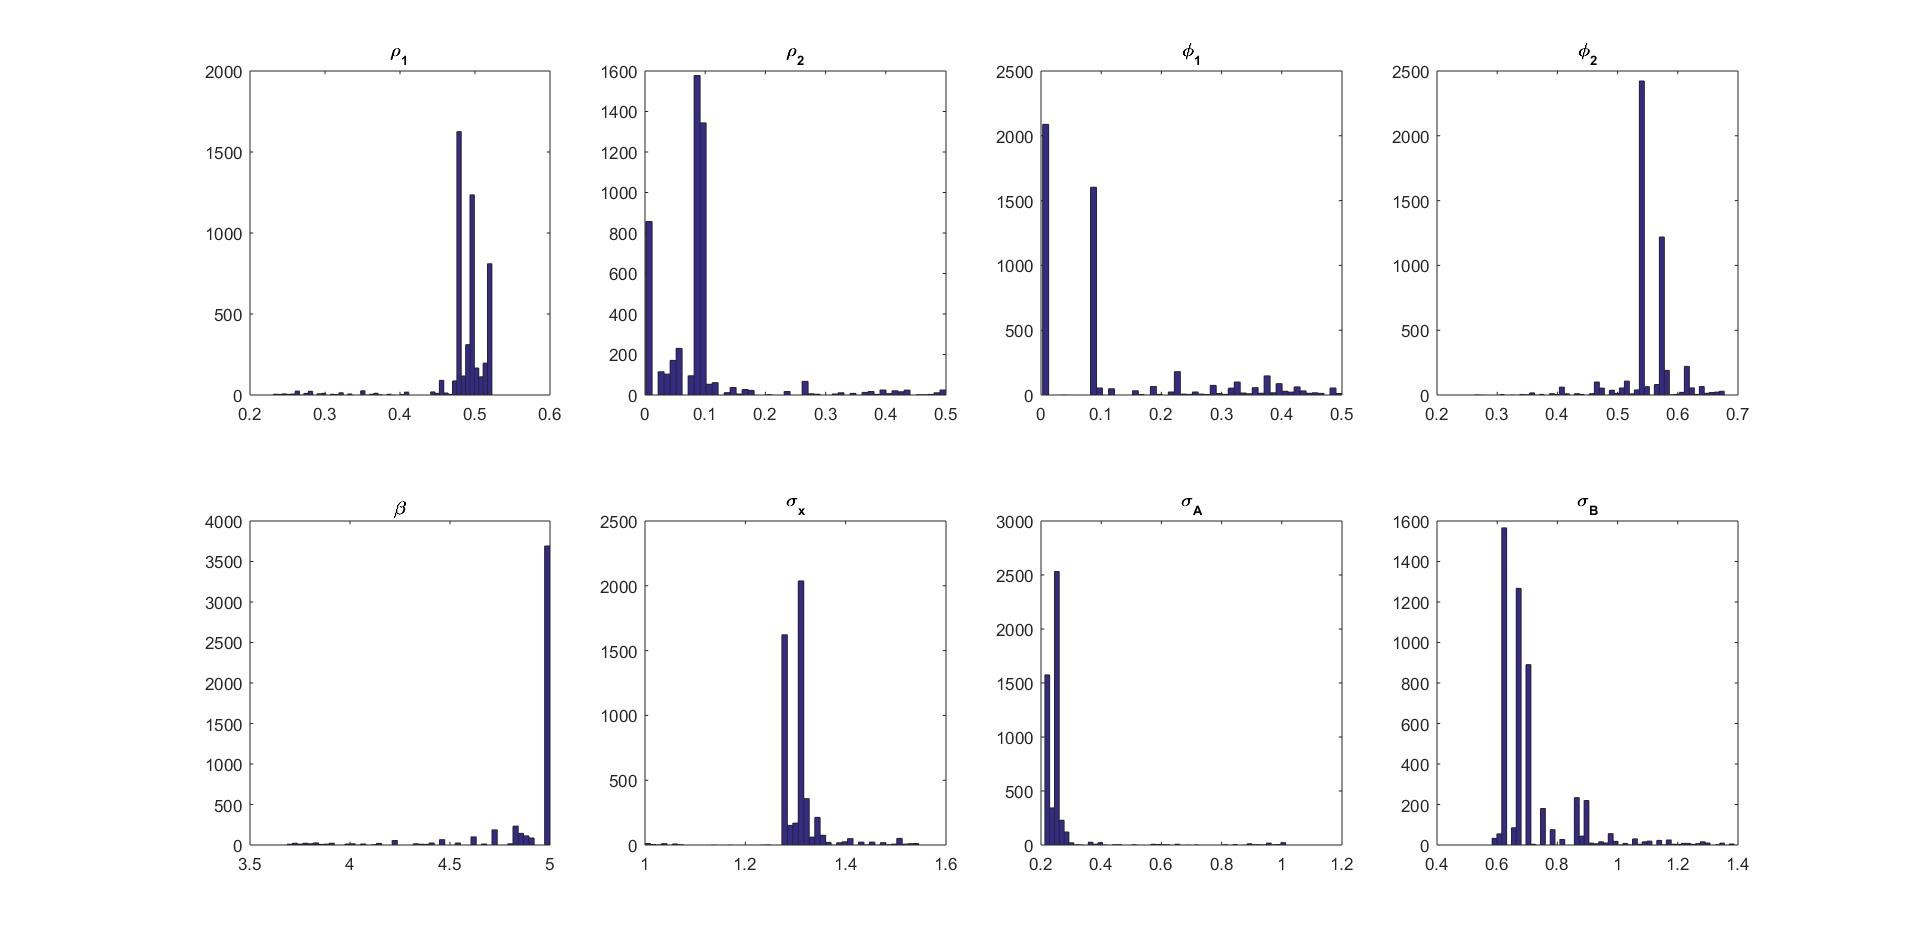
\includegraphics[scale=.38]{PosteriorDistribution.jpg}}
\caption{Posterior Distribution of $\theta$}
\end{sidewaysfigure}
\end{enumerate}

\newgeometry{left=2cm, right=2cm}
\Large {\bf Appendices}
\appendix
\section{The main program PS7\_McMc\_sampler.m}
\lstinputlisting[language=Matlab]{PS7_McMc_sampler.m}
\section{The function file PS7\_model\_llh.m}
\lstinputlisting[language=Matlab]{PS7_model_llh.m}
\restoregeometry

\end{document}